% PROPORTIONAL RELATIONSHIPS - WORKSHEET 0 (IN-CLASS INSTRUCTION)
\documentclass[12pt, letterpaper, fleqn]{article}

% ----------------------------------------------------------
% PACKAGES
% ----------------------------------------------------------
\usepackage{graphicx}
\usepackage{xcolor}
\usepackage[most]{tcolorbox}
\usepackage{amsmath, amssymb}
\usepackage{fancyhdr}
\usepackage[utf8]{inputenc}
\usepackage[T1]{fontenc}
\usepackage{enumitem}
\usepackage{geometry}
\usepackage{tikz}
\usepackage{needspace}
\usepackage{multicol}

\usetikzlibrary{arrows.meta, calc}

% ----------------------------------------------------------
% PAGE SETUP
% ----------------------------------------------------------
\usepackage{times}
\geometry{letterpaper, top=1.25in, bottom=1.25in, marginpar=0.5in}

% ----------------------------------------------------------
% HEADER / FOOTER
% ----------------------------------------------------------
\newcommand{\logowidth}{3cm}
\setlength{\headheight}{20pt}
\setlength{\footskip}{40pt}

\pagestyle{fancy}
\fancyhf{}
\fancyhead[C]{\small\bfseries Proportional Relationships}
\fancyfoot[L]{\raisebox{2pt}{
\includegraphics[width=\logowidth]{kss.png}}}
\fancyfoot[C]{\thepage}
\fancyfoot[R]{7.2.0}

\renewcommand{\footrulewidth}{0.2pt}

% ----------------------------------------------------------
% THEME COLOR
% ----------------------------------------------------------
\definecolor{customteal}{HTML}{2fbdb9}

% ----------------------------------------------------------
% HELPER MACROS
% ----------------------------------------------------------
\newcommand{\blank}{\underline{\hspace{2.2cm}}}
\newcommand{\blanklong}{\underline{\hspace{6.5cm}}}
\newcommand{\blankshorter}{\underline{\hspace{1.5cm}}}

% ----------------------------------------------------------
% DOCUMENT
% ----------------------------------------------------------
\begin{document}

\textbf{Name:} \underline{\hspace{5cm}}
\hfill
\textbf{Date:} \underline{\hspace{3cm}}\\

% ==========================================================
% SECTION 1: WHAT IS A PROPORTIONAL RELATIONSHIP?
% ==========================================================
\begin{tcolorbox}[colback=customteal!20]
    \large\textcolor{black}{\textbf{What is a Proportional Relationship?}}
\end{tcolorbox}

\vspace{3mm}

\noindent
Two quantities are in a \textbf{proportional relationship} if they have a constant ratio. This means that as one quantity changes, the other quantity changes by the same factor.

\begin{itemize}
    \item If the ratio of the two quantities is constant, the relationship is proportional.
    \item If the ratio changes, the relationship is not proportional.
\end{itemize}

\vspace{4mm}

% ==========================================================
% IDENTIFYING PROPORTIONAL RELATIONSHIPS USING TABLES
% ==========================================================
\begin{tcolorbox}[colback=customteal!10, colframe=customteal, boxrule=1pt, arc=3mm]
    \textbf{Tables:} To determine if a relationship is proportional using a table, calculate the ratio of the two quantities for each pair of values. If the ratio is the same for all pairs, the relationship is proportional. This constant ratio is called the \textbf{constant of proportionality}.
\end{tcolorbox}

\vspace{4mm}

\begin{tcolorbox}[colback=white, colframe=black!25, boxrule=0.6pt, arc=4mm, left=6mm, right=6mm, top=5mm, bottom=5mm]

\textbf{Example 1: Is it proportional?}

\medskip

\noindent
\textbf{Table A:}

\begin{tabular}{|c|c|}
\hline
$x$ & $y$ \\
\hline
2 & 4 \\
3 & 6 \\
4 & 8 \\
\hline
\end{tabular}

\medskip

\noindent
\textbf{Calculation:}
\begin{itemize}
    \item $\frac{y}{x}$ for (2, 4): $\frac{4}{2} = 2$
    \item $\frac{y}{x}$ for (3, 6): $\frac{6}{3} = 2$
    \item $\frac{y}{x}$ for (4, 8): $\frac{8}{4} = 2$
\end{itemize}
Since the ratio $\frac{y}{x}$ is constant ($2$), Table A represents a proportional relationship. The constant of proportionality is $2$.

\medskip
\noindent
\textbf{Table B:}

\begin{tabular}{|c|c|}
\hline
$x$ & $y$ \\
\hline
1 & 3 \\
2 & 5 \\
3 & 7 \\
\hline
\end{tabular}

\medskip

\noindent
\textbf{Calculation:}
\begin{itemize}
    \item $\frac{y}{x}$ for (1, 3): $\frac{3}{1} = 3$
    \item $\frac{y}{x}$ for (2, 5): $\frac{5}{2} = 2.5$
    \item $\frac{y}{x}$ for (3, 7): $\frac{7}{3} \approx 2.33$
\end{itemize}
Since the ratio $\frac{y}{x}$ is not constant, Table B does not represent a proportional relationship.

\end{tcolorbox}

\vspace{4mm}

% ==========================================================
% IDENTIFYING PROPORTIONAL RELATIONSHIPS USING GRAPHS
% ==========================================================
\begin{tcolorbox}[colback=customteal!10, colframe=customteal, boxrule=1pt, arc=3mm]
    \textbf{Graphs:} A relationship is proportional if its graph is a straight line that passes through the \textbf{origin} (0,0).
\end{tcolorbox}

\vspace{4mm}

\begin{tcolorbox}[colback=white, colframe=black!25, boxrule=0.6pt, arc=4mm, left=6mm, right=6mm, top=5mm, bottom=5mm]

\textbf{Example 2: Graphing Proportional Relationships}

\medskip

\noindent
\textbf{Graph A:} (Plotting points from Table A)
\begin{center}
\begin{tikzpicture}
    \draw[->] (-1,0) -- (5,0) node[right] {$x$};
    \draw[->] (0,-1) -- (0,9) node[above] {$y$};
    \draw[thick, customteal] (0,0) -- (1,2) -- (2,4) -- (3,6) -- (4,8);
    \fill[black] (2,4) circle (1.5pt);
    \fill[black] (3,6) circle (1.5pt);
    \fill[black] (4,8) circle (1.5pt);
    \fill[black] (1,2) circle (1.5pt);
\end{tikzpicture}
\end{center}
This graph is a straight line passing through the origin (0,0). Therefore, it represents a proportional relationship.

\medskip

\noindent
\textbf{Graph B:} (Plotting points from Table B)
\begin{center}
\begin{tikzpicture}
    \draw[->] (-1,0) -- (5,0) node[right] {$x$};
    \draw[->] (0,-1) -- (0,9) node[above] {$y$};
    \draw[thick, red] (0,3) -- (1,3) -- (2,5) -- (3,7);
    \fill[red] (1,3) circle (1.5pt);
    \fill[red] (2,5) circle (1.5pt);
    \fill[red] (3,7) circle (1.5pt);
\end{tikzpicture}
\end{center}
This graph is not a straight line and does not pass through the origin. Therefore, it does not represent a proportional relationship.

\end{tcolorbox}

\vspace{4mm}

% ==========================================================
% THE CONSTANT OF PROPORTIONALITY (k)
% ==========================================================
\begin{tcolorbox}[colback=customteal!20]
\large\textcolor{black}{\textbf{The Constant of Proportionality (k)}}
\end{tcolorbox}

\vspace{3mm}

\noindent
The \textbf{constant of proportionality}, often represented by the letter $k$, is the constant ratio between two quantities in a proportional relationship.

\begin{itemize}
    \item \textbf{In Tables:} $k = \frac{y}{x}$ for any pair of values $(x, y)$ where $x \neq 0$.
    \item \textbf{In Graphs:} $k$ is the slope of the straight line that passes through the origin.
    \item \textbf{In Equations:} The equation for a proportional relationship is always in the form $y = kx$.
    \item \textbf{In Diagrams/Verbal Descriptions:} You can often find the ratio of the two quantities to determine $k$.
\end{itemize}

\vspace{4mm}

\begin{tcolorbox}[colback=white, colframe=black!25, boxrule=0.6pt, arc=4mm, left=6mm, right=6mm, top=5mm, bottom=5mm]

\textbf{Example 3: Finding the Constant of Proportionality}

\medskip

\noindent
\textbf{a) Verbal Description:} A recipe calls for 2 cups of flour for every 3 cups of sugar.
\begin{itemize}
    \item Ratio of flour to sugar: $\frac{2 \text{ cups flour}}{3 \text{ cups sugar}} = \frac{2}{3}$.
    \item If $y$ is flour and $x$ is sugar, $k = \frac{2}{3}$. The equation is $y = \frac{2}{3}x$.
\end{itemize}

\medskip

\noindent
\textbf{b) Diagram:}
\begin{center}
\begin{tikzpicture}
    \draw (0,0) rectangle (1,3);
    \node at (0.5, 1.5) {$5$ apples};
    \draw (2,0) rectangle (3,3);
    \node at (2.5, 1.5) {$10$ apples};
\end{tikzpicture}
\end{center}
This diagram shows that 5 apples cost $5$ dollars, and 10 apples cost $10$ dollars.
\begin{itemize}
    \item Ratio of cost to apples: $\frac{\$5}{5 \text{ apples}} = \frac{\$1}{\text{apple}}$.
    \item If $y$ is cost and $x$ is the number of apples, $k = 1$. The equation is $y = 1x$ or $y=x$.
\end{itemize}

\medskip

\noindent
\textbf{c) Equation:} $y = 5x$
\begin{itemize}
    \item This equation is in the form $y=kx$.
    \item The constant of proportionality is $k=5$. This means for every 1 unit of $x$, $y$ increases by 5.
\end{itemize}

\end{tcolorbox}

\vspace{4mm}

% ==========================================================
% PRACTICE 1: IDENTIFYING PROPORTIONAL RELATIONSHIPS
% ==========================================================
\newpage
\begin{tcolorbox}[colback=customteal!20]
\large\textcolor{black}{\textbf{Practice 1: Is it Proportional?}}
\end{tcolorbox}

\noindent
For each table and graph, determine if the relationship is proportional. If it is, identify the constant of proportionality ($k$).

\vspace{3mm}

\begin{enumerate}[itemsep=1.5cm, leftmargin=0.6cm]

\item \textbf{Table C:}
\begin{tabular}{|c|c|}
\hline
$x$ & $y$ \\
\hline
1 & 5 \\
2 & 10 \\
3 & 15 \\
\hline
\end{tabular}

\begin{itemize}
    \item Is it proportional? \blank
    \item If yes, $k = $ \blank
\end{itemize}

\item \textbf{Table D:}
\begin{tabular}{|c|c|}
\hline
$x$ & $y$ \\
\hline
4 & 8 \\
6 & 12 \\
8 & 14 \\
\hline
\end{tabular}

\begin{itemize}
    \item Is it proportional? \blank
    \item If yes, $k = $ \blank
\end{itemize}

\item \textbf{Graph A:} (A straight line passing through the origin)
\begin{center}
\begin{tikzpicture}
    \draw[->] (-1,0) -- (5,0) node[right] {$x$};
    \draw[->] (0,-1) -- (0,5) node[above] {$y$};
    \draw[thick, customteal] (0,0) -- (1,1) -- (2,2) -- (3,3) -- (4,4);
    \fill[black] (1,1) circle (1.5pt);
    \fill[black] (2,2) circle (1.5pt);
    \fill[black] (3,3) circle (1.5pt);
    \fill[black] (4,4) circle (1.5pt);
\end{tikzpicture}
\end{center}

\begin{itemize}
    \item Is it proportional? \blank
    \item If yes, $k = $ \blank
\end{itemize}

\item \textbf{Graph B:} (A straight line that does NOT pass through the origin)
\begin{center}
\begin{tikzpicture}
    \draw[->] (-1,0) -- (5,0) node[right] {$x$};
    \draw[->] (0,-1) -- (0,5) node[above] {$y$};
    \draw[thick, red] (1,1) -- (2,2) -- (3,3) -- (4,4);
    \fill[red] (1,1) circle (1.5pt);
    \fill[red] (2,2) circle (1.5pt);
    \fill[red] (3,3) circle (1.5pt);
    \fill[red] (4,4) circle (1.5pt);
\end{tikzpicture}
\end{center}

\begin{itemize}
    \item Is it proportional? \blank
    \item If yes, $k = $ \blank
\end{itemize}

\end{enumerate}

\newpage

% ==========================================================
% PRACTICE 2: FINDING THE CONSTANT OF PROPORTIONALITY
% ==========================================================
\begin{tcolorbox}[colback=customteal!20]
\large\textcolor{black}{\textbf{Practice 2: Finding the Constant of Proportionality (k)}}
\end{tcolorbox}

\noindent
Find the constant of proportionality ($k$) for each situation.

\vspace{3mm}

\begin{enumerate}[itemsep=1.5cm, leftmargin=0.6cm]

\item \textbf{Verbal Description:} It takes 3 hours to travel 180 miles.
\begin{itemize}
    \item $k = $ \blank miles per hour
\end{itemize}

\item \textbf{Verbal Description:} A store sells 5 notebooks for $15.
\begin{itemize}
    \item $k = $ \blank dollars per notebook
\end{itemize}

\item \textbf{Table E:}
\begin{tabular}{|c|c|}
\hline
Minutes & Steps \\
\hline
10 & 1000 \\
15 & 1500 \\
20 & 2000 \\
\hline
\end{tabular}
\begin{itemize}
    \item $k = $ \blank steps per minute
\end{itemize}

\item \textbf{Equation:} $y = 7x$
\begin{itemize}
    \item $k = $ \blank
\end{itemize}

\item \textbf{Equation:} $y = \frac{1}{4}x$
\begin{itemize}
    \item $k = $ \blank
\end{itemize}

\item \textbf{Diagram:}
\begin{center}
\begin{tikzpicture}
    \draw (0,0) rectangle (1,2);
    \node at (0.5, 1) {$4$ cookies};
    \draw (2,0) rectangle (3,2);
    \node at (2.5, 1) {$8$ cookies};
\end{center}
Assume the cost is proportional to the number of cookies.
\begin{itemize}
    \item $k = $ \blank dollars per cookie
\end{itemize}

\end{enumerate}

\end{document}